% !TEX root = main.tex
%%%%%%%%%%%%%%%%%%%%%%%%%%%%%%%%%%%%%%%%%%%%%%%%%%%%%%
\section{実験方法および結果}
%%%%%%%%%%%%%%%%%%%%%%%%%%%%%%%%%%%%%%%%%%%%%%%%%%%%%%
\subsection{Duty比100\%・Duty比50\%による制御}
\subsubsection{実験方法}
\subsubsection{実験結果}

\begin{figure}[H]
	\centering
		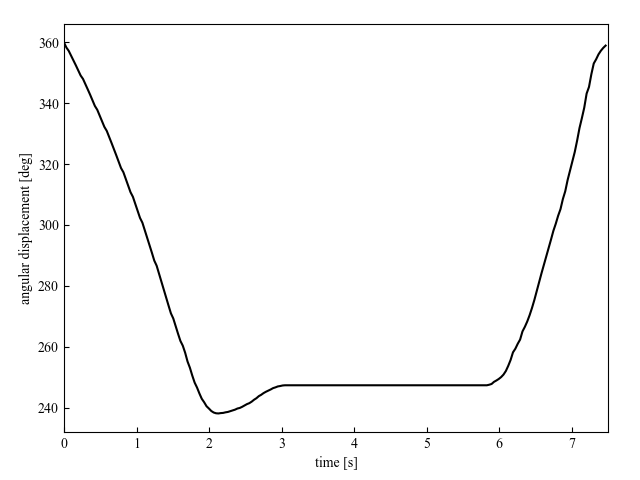
\includegraphics[scale=0.5]{./figure/5kb.png}
		\caption{50\%としたときの結果}
		\label{fig:fif}
\end{figure}

\begin{figure}[H]
	\centering
		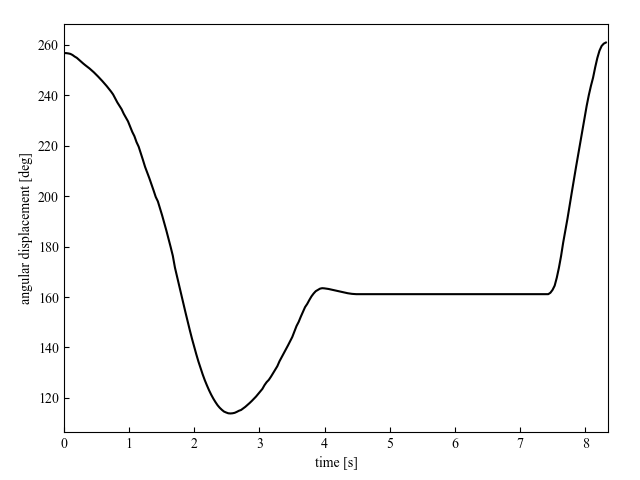
\includegraphics[scale=0.5]{./figure/fif.png}
		\caption{100\%としたときの結果}
		\label{fig:hund}
\end{figure}

\newpage

\subsection{P制御}
\subsubsection{実験方法}
\subsubsection{実験結果}

\begin{figure}[H]
	\centering
		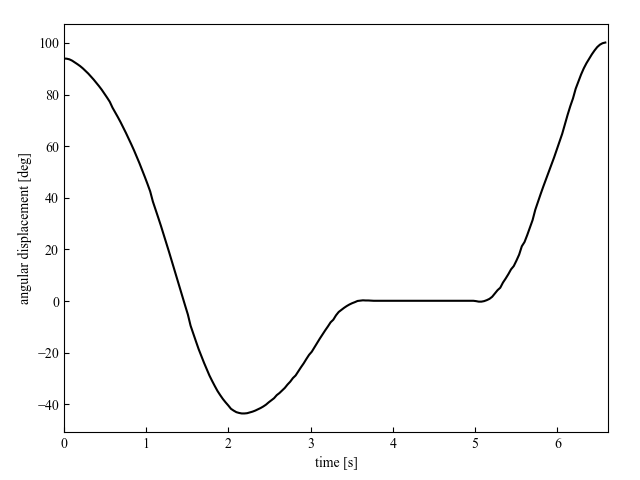
\includegraphics[scale=0.5]{./figure/P.png}
		\caption{P制御の結果}
		\label{fig:P}
\end{figure}

\newpage

\subsection{P-D制御}
\subsubsection{実験方法}
\subsubsection{実験結果}

\begin{figure}[H]
	\centering
		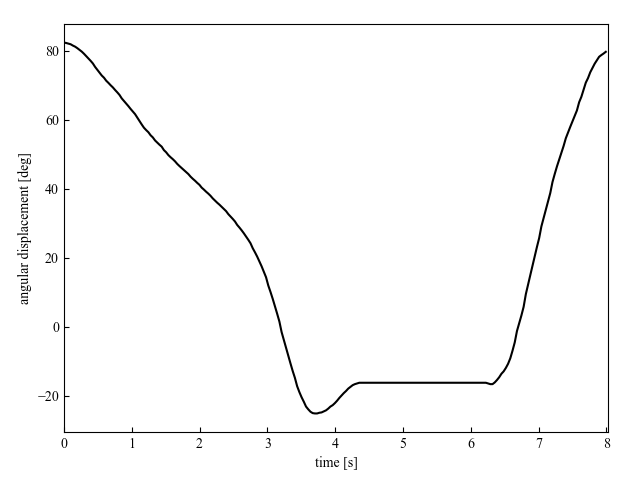
\includegraphics[scale=0.5]{./figure/PD.png}
		\caption{P-D制御の結果}
		\label{fig:PD}
\end{figure}

\newpage

\subsection{B-dot制御則}
\subsubsection{実験方法}
\subsubsection{実験結果}

\begin{figure}[H]
	\centering
		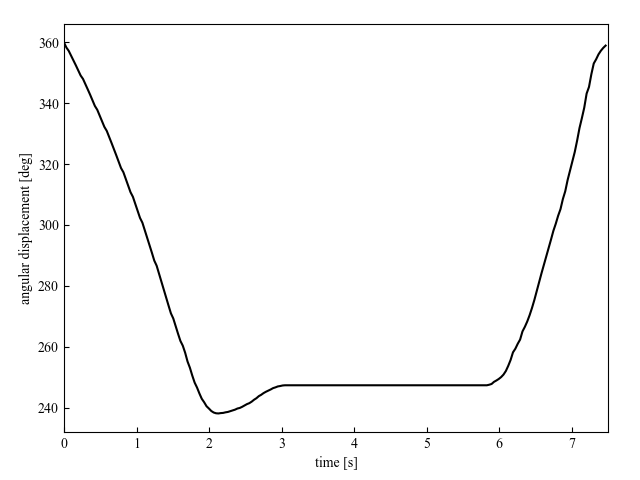
\includegraphics[scale=0.5]{./figure/5kb.png}
		\caption{kb = 0.0005としたときの結果}
		\label{fig:kb5}
\end{figure}

\begin{figure}[H]
	\centering
		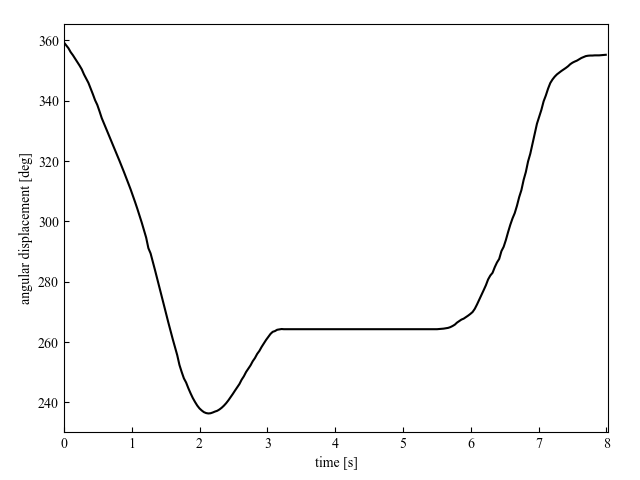
\includegraphics[scale=0.5]{./figure/15kb.png}
		\caption{kb = 0.0015としたときの結果}
		\label{fig:kb15}
\end{figure}

\newpage

\subsection{クロスプロダクト則}
\subsubsection{実験方法}
\subsubsection{実験結果}

\begin{figure}[H]
	\centering
		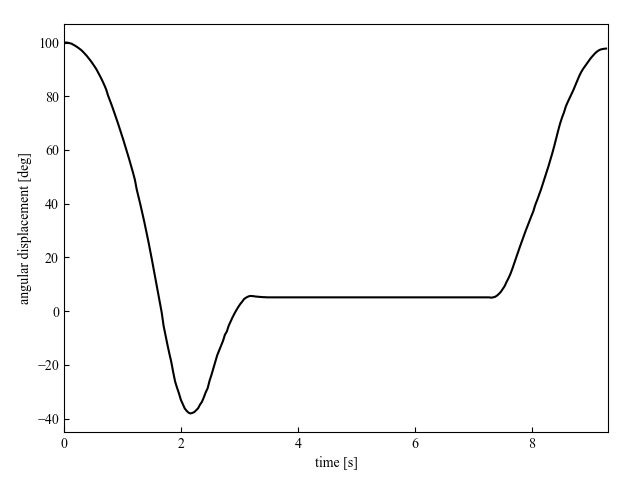
\includegraphics[scale=0.5]{./figure/cross.png}
		\caption{結果}
		\label{fig:cross}
\end{figure}

\subsection{考察}

\newpage
\section{結論}
\subsection{本研究のまとめ}
\subsection{今後の展望}